\documentclass{standalone}
\usepackage{tikz}
\usetikzlibrary{patterns, positioning}


\begin{document}
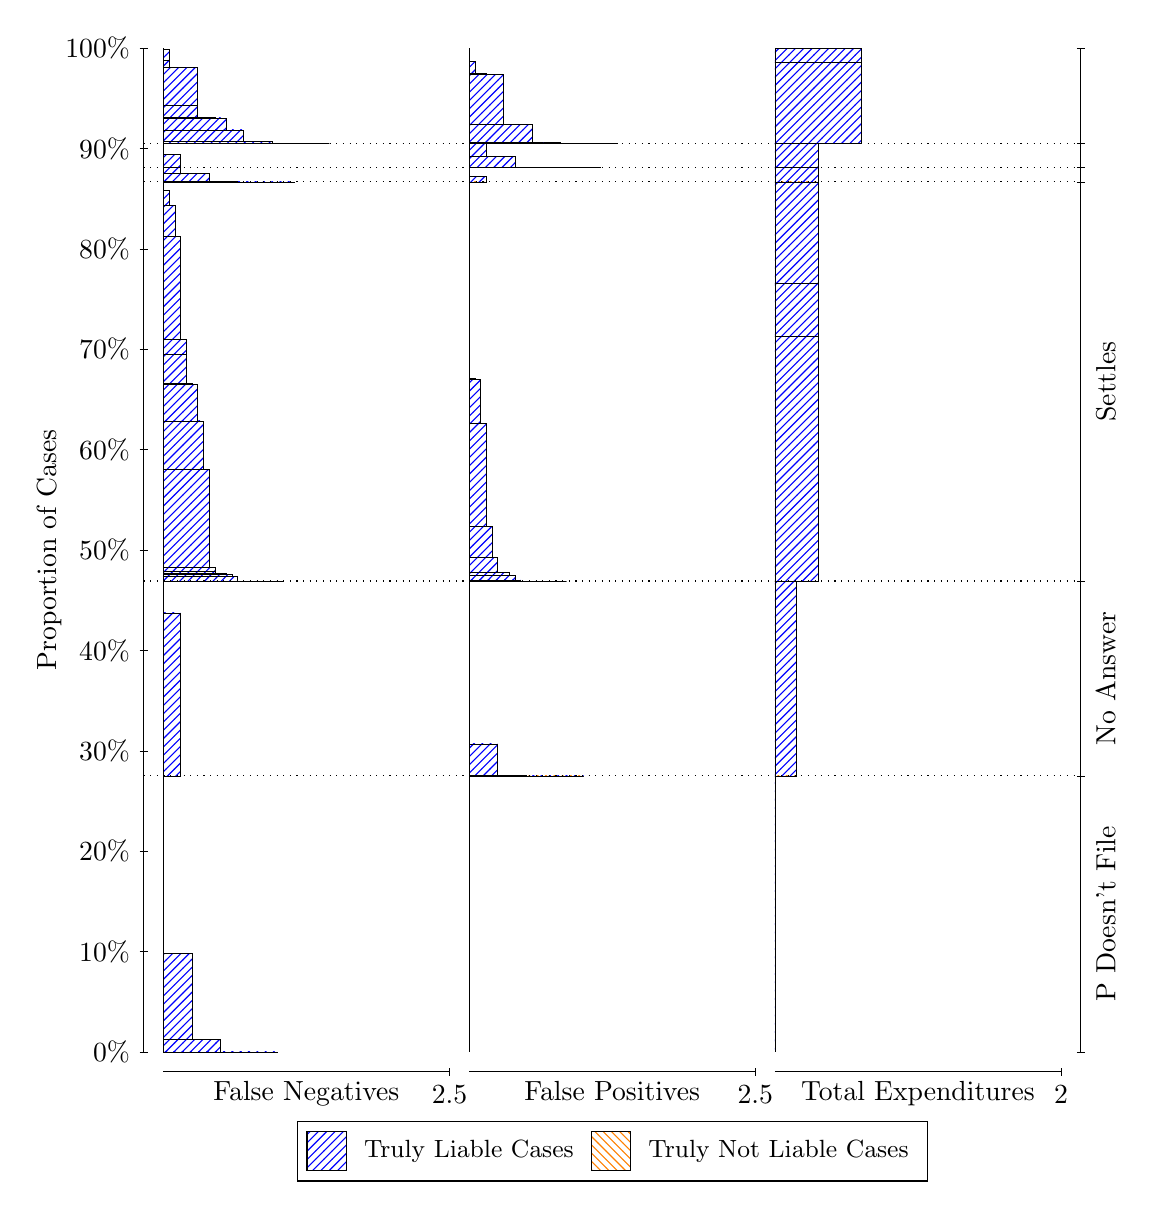
\begin{tikzpicture}
\draw[black, very thin] (1.5,1.75) -- (1.5,14.5);
\node[rotate=90, text=black, anchor=center] at (0.3, 8.125) {Proportion of Cases};
\draw[black, very thin] (1.45,1.75) -- (1.55,1.75);
\node[text=black, anchor=east] at (1.45, 1.75) {0\%};
\draw[black, very thin] (1.45,3.025) -- (1.55,3.025);
\node[text=black, anchor=east] at (1.45, 3.025) {10\%};
\draw[black, very thin] (1.45,4.3) -- (1.55,4.3);
\node[text=black, anchor=east] at (1.45, 4.3) {20\%};
\draw[black, very thin] (1.45,5.575) -- (1.55,5.575);
\node[text=black, anchor=east] at (1.45, 5.575) {30\%};
\draw[black, very thin] (1.45,6.85) -- (1.55,6.85);
\node[text=black, anchor=east] at (1.45, 6.85) {40\%};
\draw[black, very thin] (1.45,8.125) -- (1.55,8.125);
\node[text=black, anchor=east] at (1.45, 8.125) {50\%};
\draw[black, very thin] (1.45,9.4) -- (1.55,9.4);
\node[text=black, anchor=east] at (1.45, 9.4) {60\%};
\draw[black, very thin] (1.45,10.675) -- (1.55,10.675);
\node[text=black, anchor=east] at (1.45, 10.675) {70\%};
\draw[black, very thin] (1.45,11.95) -- (1.55,11.95);
\node[text=black, anchor=east] at (1.45, 11.95) {80\%};
\draw[black, very thin] (1.45,13.225) -- (1.55,13.225);
\node[text=black, anchor=east] at (1.45, 13.225) {90\%};
\draw[black, very thin] (1.45,14.5) -- (1.55,14.5);
\node[text=black, anchor=east] at (1.45, 14.5) {100\%};

\draw[black, very thin] (13.4,1.75) -- (13.4,14.5);
\draw[black, very thin] (13.35,1.75) -- (13.45,1.75);
\node[anchor=west] at (13.35, 1.75) {};
\draw[black, very thin] (13.35,5.257) -- (13.45,5.257);
\node[anchor=west] at (13.35, 5.257) {};
\draw[black, very thin] (13.35,7.7308) -- (13.45,7.7308);
\node[anchor=west] at (13.35, 7.7308) {};
\draw[black, very thin] (13.35,12.801) -- (13.45,12.801);
\node[anchor=west] at (13.35, 12.801) {};
\draw[black, very thin] (13.35,12.982) -- (13.45,12.982);
\node[anchor=west] at (13.35, 12.982) {};
\draw[black, very thin] (13.35,13.29) -- (13.45,13.29);
\node[anchor=west] at (13.35, 13.29) {};
\draw[black, very thin] (13.35,14.5) -- (13.45,14.5);
\node[anchor=west] at (13.35, 14.5) {};

\draw[black, very thin, pattern color=blue, pattern=north east lines] (1.75,1.75) rectangle (3.2033,1.75);
\draw[black, very thin, pattern color=blue, pattern=north east lines] (1.75,1.75) rectangle (2.84,1.7514);
\draw[black, very thin, pattern color=blue, pattern=north east lines] (1.75,1.7514) rectangle (2.4767,1.9127);
\draw[black, very thin, pattern color=blue, pattern=north east lines] (1.75,1.9127) rectangle (2.1133,3.0003);
\draw[black, very thin, pattern color=orange, pattern=north west lines] (1.75,3.0003) rectangle (1.75,3.0003);
\draw[black, very thin, pattern color=blue, pattern=north east lines] (1.75,3.0003) rectangle (1.75,5.257);
\draw[black, very thin, pattern color=blue, pattern=north east lines] (1.75,5.257) rectangle (1.968,7.3261);
\draw[black, very thin, pattern color=orange, pattern=north west lines] (1.75,7.3261) rectangle (1.75,7.3261);
\draw[black, very thin, pattern color=blue, pattern=north east lines] (1.75,7.3261) rectangle (1.75,7.7308);
\draw[black, very thin, pattern color=blue, pattern=north east lines] (1.75,7.7308) rectangle (3.276,7.7308);
\draw[black, very thin, pattern color=blue, pattern=north east lines] (1.75,7.7308) rectangle (3.1307,7.7308);
\draw[black, very thin, pattern color=blue, pattern=north east lines] (1.75,7.7308) rectangle (2.9853,7.7308);
\draw[black, very thin, pattern color=blue, pattern=north east lines] (1.75,7.7308) rectangle (2.9127,7.7308);
\draw[black, very thin, pattern color=blue, pattern=north east lines] (1.75,7.7308) rectangle (2.84,7.7308);
\draw[black, very thin, pattern color=blue, pattern=north east lines] (1.75,7.7308) rectangle (2.7673,7.7309);
\draw[black, very thin, pattern color=blue, pattern=north east lines] (1.75,7.7309) rectangle (2.6947,7.7885);
\draw[black, very thin, pattern color=blue, pattern=north east lines] (1.75,7.7885) rectangle (2.622,7.8106);
\draw[black, very thin, pattern color=blue, pattern=north east lines] (1.75,7.8106) rectangle (2.5493,7.8292);
\draw[black, very thin, pattern color=blue, pattern=north east lines] (1.75,7.8292) rectangle (2.4767,7.8296);
\draw[black, very thin, pattern color=blue, pattern=north east lines] (1.75,7.8296) rectangle (2.404,7.8577);
\draw[black, very thin, pattern color=blue, pattern=north east lines] (1.75,7.8577) rectangle (2.404,7.9089);
\draw[black, very thin, pattern color=blue, pattern=north east lines] (1.75,7.9089) rectangle (2.3313,9.1533);
\draw[black, very thin, pattern color=blue, pattern=north east lines] (1.75,9.1533) rectangle (2.2587,9.7638);
\draw[black, very thin, pattern color=blue, pattern=north east lines] (1.75,9.7638) rectangle (2.186,10.229);
\draw[black, very thin, pattern color=blue, pattern=north east lines] (1.75,10.229) rectangle (2.1133,10.24);
\draw[black, very thin, pattern color=blue, pattern=north east lines] (1.75,10.24) rectangle (2.0407,10.616);
\draw[black, very thin, pattern color=blue, pattern=north east lines] (1.75,10.616) rectangle (2.0407,10.797);
\draw[black, very thin, pattern color=blue, pattern=north east lines] (1.75,10.797) rectangle (1.968,12.11);
\draw[black, very thin, pattern color=blue, pattern=north east lines] (1.75,12.11) rectangle (1.8953,12.501);
\draw[black, very thin, pattern color=blue, pattern=north east lines] (1.75,12.501) rectangle (1.8227,12.694);
\draw[black, very thin, pattern color=blue, pattern=north east lines] (1.75,12.694) rectangle (1.75,12.695);
\draw[black, very thin, pattern color=orange, pattern=north west lines] (1.75,12.695) rectangle (1.75,12.695);
\draw[black, very thin, pattern color=blue, pattern=north east lines] (1.75,12.695) rectangle (1.75,12.801);
\draw[black, very thin, pattern color=blue, pattern=north east lines] (1.75,12.801) rectangle (3.4213,12.801);
\draw[black, very thin, pattern color=blue, pattern=north east lines] (1.75,12.801) rectangle (3.058,12.801);
\draw[black, very thin, pattern color=blue, pattern=north east lines] (1.75,12.801) rectangle (2.6947,12.805);
\draw[black, very thin, pattern color=blue, pattern=north east lines] (1.75,12.805) rectangle (2.3313,12.911);
\draw[black, very thin, pattern color=blue, pattern=north east lines] (1.75,12.911) rectangle (1.968,12.982);
\draw[black, very thin, pattern color=orange, pattern=north west lines] (1.75,12.982) rectangle (1.75,12.982);
\draw[black, very thin, pattern color=blue, pattern=north east lines] (1.75,12.982) rectangle (1.968,13.147);
\draw[black, very thin, pattern color=orange, pattern=north west lines] (1.75,13.147) rectangle (1.75,13.147);
\draw[black, very thin, pattern color=blue, pattern=north east lines] (1.75,13.147) rectangle (1.75,13.29);
\draw[black, very thin, pattern color=blue, pattern=north east lines] (1.75,13.29) rectangle (3.8573,13.29);
\draw[black, very thin, pattern color=blue, pattern=north east lines] (1.75,13.29) rectangle (3.494,13.291);
\draw[black, very thin, pattern color=blue, pattern=north east lines] (1.75,13.291) rectangle (3.276,13.291);
\draw[black, very thin, pattern color=blue, pattern=north east lines] (1.75,13.291) rectangle (3.1307,13.314);
\draw[black, very thin, pattern color=blue, pattern=north east lines] (1.75,13.314) rectangle (2.9127,13.314);
\draw[black, very thin, pattern color=blue, pattern=north east lines] (1.75,13.314) rectangle (2.7673,13.46);
\draw[black, very thin, pattern color=blue, pattern=north east lines] (1.75,13.46) rectangle (2.5493,13.612);
\draw[black, very thin, pattern color=blue, pattern=north east lines] (1.75,13.612) rectangle (2.404,13.622);
\draw[black, very thin, pattern color=blue, pattern=north east lines] (1.75,13.622) rectangle (2.186,13.774);
\draw[black, very thin, pattern color=blue, pattern=north east lines] (1.75,13.774) rectangle (2.186,14.257);
\draw[black, very thin, pattern color=blue, pattern=north east lines] (1.75,14.257) rectangle (2.0407,14.257);
\draw[black, very thin, pattern color=blue, pattern=north east lines] (1.75,14.257) rectangle (1.8227,14.342);
\draw[black, very thin, pattern color=blue, pattern=north east lines] (1.75,14.342) rectangle (1.8227,14.486);
\draw[black, very thin, pattern color=orange, pattern=north west lines] (1.75,14.486) rectangle (1.75,14.486);
\draw[black, very thin, pattern color=blue, pattern=north east lines] (1.75,14.486) rectangle (1.75,14.5);
\draw[black, very thin, pattern color=orange, pattern=north west lines] (5.6333,1.75) rectangle (5.6333,1.75);
\draw[black, very thin, pattern color=blue, pattern=north east lines] (5.6333,1.75) rectangle (5.6333,5.257);
\draw[black, very thin, pattern color=orange, pattern=north west lines] (5.6333,5.257) rectangle (7.0867,5.257);
\draw[black, very thin, pattern color=blue, pattern=north east lines] (5.6333,5.257) rectangle (7.0867,5.257);
\draw[black, very thin, pattern color=blue, pattern=north east lines] (5.6333,5.257) rectangle (6.7233,5.257);
\draw[black, very thin, pattern color=blue, pattern=north east lines] (5.6333,5.257) rectangle (6.36,5.2602);
\draw[black, very thin, pattern color=blue, pattern=north east lines] (5.6333,5.2602) rectangle (5.9967,5.6617);
\draw[black, very thin, pattern color=blue, pattern=north east lines] (5.6333,5.6617) rectangle (5.6333,7.7308);
\draw[black, very thin, pattern color=orange, pattern=north west lines] (5.6333,7.7308) rectangle (6.8687,7.7308);
\draw[black, very thin, pattern color=blue, pattern=north east lines] (5.6333,7.7308) rectangle (6.8687,7.7308);
\draw[black, very thin, pattern color=orange, pattern=north west lines] (5.6333,7.7308) rectangle (6.578,7.7308);
\draw[black, very thin, pattern color=blue, pattern=north east lines] (5.6333,7.7308) rectangle (6.578,7.7308);
\draw[black, very thin, pattern color=blue, pattern=north east lines] (5.6333,7.7308) rectangle (6.5053,7.7308);
\draw[black, very thin, pattern color=orange, pattern=north west lines] (5.6333,7.7308) rectangle (6.4327,7.7308);
\draw[black, very thin, pattern color=blue, pattern=north east lines] (5.6333,7.7308) rectangle (6.4327,7.7308);
\draw[black, very thin, pattern color=orange, pattern=north west lines] (5.6333,7.7308) rectangle (6.2873,7.7308);
\draw[black, very thin, pattern color=blue, pattern=north east lines] (5.6333,7.7308) rectangle (6.2873,7.7449);
\draw[black, very thin, pattern color=blue, pattern=north east lines] (5.6333,7.7449) rectangle (6.2147,7.8072);
\draw[black, very thin, pattern color=orange, pattern=north west lines] (5.6333,7.8072) rectangle (6.142,7.8072);
\draw[black, very thin, pattern color=blue, pattern=north east lines] (5.6333,7.8072) rectangle (6.142,7.8375);
\draw[black, very thin, pattern color=blue, pattern=north east lines] (5.6333,7.8375) rectangle (6.0693,7.8379);
\draw[black, very thin, pattern color=orange, pattern=north west lines] (5.6333,7.8379) rectangle (5.9967,7.8379);
\draw[black, very thin, pattern color=blue, pattern=north east lines] (5.6333,7.8379) rectangle (5.9967,8.0316);
\draw[black, very thin, pattern color=blue, pattern=north east lines] (5.6333,8.0316) rectangle (5.924,8.4221);
\draw[black, very thin, pattern color=blue, pattern=north east lines] (5.6333,8.4221) rectangle (5.8513,9.735);
\draw[black, very thin, pattern color=blue, pattern=north east lines] (5.6333,9.735) rectangle (5.7787,10.293);
\draw[black, very thin, pattern color=blue, pattern=north east lines] (5.6333,10.293) rectangle (5.706,10.303);
\draw[black, very thin, pattern color=blue, pattern=north east lines] (5.6333,10.303) rectangle (5.6333,12.801);
\draw[black, very thin, pattern color=orange, pattern=north west lines] (5.6333,12.801) rectangle (5.8513,12.801);
\draw[black, very thin, pattern color=blue, pattern=north east lines] (5.6333,12.801) rectangle (5.8513,12.873);
\draw[black, very thin, pattern color=blue, pattern=north east lines] (5.6333,12.873) rectangle (5.6333,12.982);
\draw[black, very thin, pattern color=orange, pattern=north west lines] (5.6333,12.982) rectangle (7.3047,12.982);
\draw[black, very thin, pattern color=blue, pattern=north east lines] (5.6333,12.982) rectangle (7.3047,12.982);
\draw[black, very thin, pattern color=blue, pattern=north east lines] (5.6333,12.982) rectangle (6.9413,12.982);
\draw[black, very thin, pattern color=blue, pattern=north east lines] (5.6333,12.982) rectangle (6.578,12.984);
\draw[black, very thin, pattern color=blue, pattern=north east lines] (5.6333,12.984) rectangle (6.2147,13.125);
\draw[black, very thin, pattern color=blue, pattern=north east lines] (5.6333,13.125) rectangle (5.8513,13.29);
\draw[black, very thin, pattern color=orange, pattern=north west lines] (5.6333,13.29) rectangle (7.5227,13.29);
\draw[black, very thin, pattern color=blue, pattern=north east lines] (5.6333,13.29) rectangle (7.5227,13.29);
\draw[black, very thin, pattern color=orange, pattern=north west lines] (5.6333,13.29) rectangle (7.1593,13.29);
\draw[black, very thin, pattern color=blue, pattern=north east lines] (5.6333,13.29) rectangle (7.1593,13.291);
\draw[black, very thin, pattern color=orange, pattern=north west lines] (5.6333,13.291) rectangle (6.796,13.291);
\draw[black, very thin, pattern color=blue, pattern=north east lines] (5.6333,13.291) rectangle (6.796,13.305);
\draw[black, very thin, pattern color=orange, pattern=north west lines] (5.6333,13.305) rectangle (6.578,13.305);
\draw[black, very thin, pattern color=blue, pattern=north east lines] (5.6333,13.305) rectangle (6.578,13.305);
\draw[black, very thin, pattern color=orange, pattern=north west lines] (5.6333,13.305) rectangle (6.4327,13.305);
\draw[black, very thin, pattern color=blue, pattern=north east lines] (5.6333,13.305) rectangle (6.4327,13.533);
\draw[black, very thin, pattern color=orange, pattern=north west lines] (5.6333,13.533) rectangle (6.2147,13.533);
\draw[black, very thin, pattern color=blue, pattern=north east lines] (5.6333,13.533) rectangle (6.2147,13.533);
\draw[black, very thin, pattern color=blue, pattern=north east lines] (5.6333,13.533) rectangle (6.0693,14.169);
\draw[black, very thin, pattern color=blue, pattern=north east lines] (5.6333,14.169) rectangle (5.8513,14.176);
\draw[black, very thin, pattern color=orange, pattern=north west lines] (5.6333,14.176) rectangle (5.8513,14.176);
\draw[black, very thin, pattern color=blue, pattern=north east lines] (5.6333,14.176) rectangle (5.8513,14.178);
\draw[black, very thin, pattern color=blue, pattern=north east lines] (5.6333,14.178) rectangle (5.706,14.331);
\draw[black, very thin, pattern color=blue, pattern=north east lines] (5.6333,14.331) rectangle (5.6333,14.5);
\draw[black, very thin, pattern color=orange, pattern=north west lines] (9.5167,1.75) rectangle (9.5167,1.75);
\draw[black, very thin, pattern color=blue, pattern=north east lines] (9.5167,1.75) rectangle (9.5167,5.257);
\draw[black, very thin, pattern color=orange, pattern=north west lines] (9.5167,5.257) rectangle (9.7892,5.257);
\draw[black, very thin, pattern color=blue, pattern=north east lines] (9.5167,5.257) rectangle (9.7892,7.7308);
\draw[black, very thin, pattern color=orange, pattern=north west lines] (9.5167,7.7308) rectangle (10.062,7.7308);
\draw[black, very thin, pattern color=blue, pattern=north east lines] (9.5167,7.7308) rectangle (10.062,10.833);
\draw[black, very thin, pattern color=orange, pattern=north west lines] (9.5167,10.833) rectangle (10.062,10.833);
\draw[black, very thin, pattern color=blue, pattern=north east lines] (9.5167,10.833) rectangle (10.062,11.511);
\draw[black, very thin, pattern color=orange, pattern=north west lines] (9.5167,11.511) rectangle (10.062,11.511);
\draw[black, very thin, pattern color=blue, pattern=north east lines] (9.5167,11.511) rectangle (10.062,12.801);
\draw[black, very thin, pattern color=orange, pattern=north west lines] (9.5167,12.801) rectangle (10.062,12.801);
\draw[black, very thin, pattern color=blue, pattern=north east lines] (9.5167,12.801) rectangle (10.062,12.982);
\draw[black, very thin, pattern color=orange, pattern=north west lines] (9.5167,12.982) rectangle (10.062,12.982);
\draw[black, very thin, pattern color=blue, pattern=north east lines] (9.5167,12.982) rectangle (10.062,13.29);
\draw[black, very thin, pattern color=orange, pattern=north west lines] (9.5167,13.29) rectangle (10.607,13.29);
\draw[black, very thin, pattern color=blue, pattern=north east lines] (9.5167,13.29) rectangle (10.607,14.321);
\draw[black, very thin, pattern color=orange, pattern=north west lines] (9.5167,14.321) rectangle (10.607,14.321);
\draw[black, very thin, pattern color=blue, pattern=north east lines] (9.5167,14.321) rectangle (10.607,14.5);
\draw[black, dotted] (1.5,5.257) -- (13.4,5.257);
\draw[black, dotted] (1.5,7.7308) -- (13.4,7.7308);
\draw[black, dotted] (1.5,12.801) -- (13.4,12.801);
\draw[black, dotted] (1.5,12.982) -- (13.4,12.982);
\draw[black, dotted] (1.5,13.29) -- (13.4,13.29);
\draw[black, very thin] (1.75,1.5) -- (5.3833,1.5);
\node[text=black, anchor=north] at (3.5667, 1.5) {False Negatives};
\draw[black, very thin] (5.3833,1.45) -- (5.3833,1.55);
\node[text=black, anchor=north] at (5.3833, 1.45) {2.5};

\draw[black, very thin] (5.6333,1.5) -- (9.2667,1.5);
\node[text=black, anchor=north] at (7.45, 1.5) {False Positives};
\draw[black, very thin] (9.2667,1.45) -- (9.2667,1.55);
\node[text=black, anchor=north] at (9.2667, 1.45) {2.5};

\draw[black, very thin] (9.5167,1.5) -- (13.15,1.5);
\node[text=black, anchor=north] at (11.333, 1.5) {Total Expenditures};
\draw[black, very thin] (13.15,1.45) -- (13.15,1.55);
\node[text=black, anchor=north] at (13.15, 1.45) {2};

\node[text=black, centered, rotate=90] at (13.72, 3.5035) {P Doesn't File};
\node[text=black, centered, rotate=90] at (13.72, 6.4939) {No Answer};
\node[text=black, centered, rotate=90] at (13.72, 10.266) {Settles};




\draw (7.449999999999999,1.5) node[draw=none] (baseCoordinate) {};
\begin{scope}[align=center]
        \matrix[scale=0.5, draw=black, below=0.5cm of baseCoordinate, nodes={draw}, column sep=0.1cm]{
            \node[rectangle, draw, minimum width=0.5cm, minimum height=0.5cm, pattern color=blue, pattern=north east lines] {}; &
            \node[draw=none, font=\small, text=black] (B) {Truly Liable Cases}; &
            \node[rectangle, draw, minimum width=0.5cm, minimum height=0.5cm, pattern color=orange, pattern=north west lines] {}; &
            \node[draw=none, font=\small, text=black] (B) {Truly Not Liable Cases}; \\
            };
\end{scope}

\end{tikzpicture}
\end{document}